% Adjust these for the path of the theme and its graphics, relative to this file
%\usepackage{beamerthemeFalmouthGamesAcademy}
\usepackage{../../beamerthemeFalmouthGamesAcademy}
\usepackage{multimedia}
\graphicspath{ {../../} }

% Default language for code listings
\lstset{language=C++,
        morekeywords={each,in,nullptr}
}

% For strikethrough effect
\usepackage[normalem]{ulem}
\usepackage{wasysym}

\usepackage{algpseudocode}

\usepackage{pdfpages}

% http://www.texample.net/tikz/examples/state-machine/
\usetikzlibrary{arrows,automata}

\usepackage{qtree}

\newcommand{\modulecode}{COMP260}\newcommand{\moduletitle}{Distributed Systems}\newcommand{\sessionnumber}{5}

\begin{document}
\title{\sessionnumber: Designing AI behaviours}
\subtitle{\modulecode: \moduletitle}

\frame{\titlepage} 

\begin{frame}
	\frametitle{Learning outcomes}
	\begin{itemize}
		\item \textbf{Explain} how finite state machines and behaviour trees are used in AI
        \item \textbf{Design} character behaviours using behaviour trees
        \item \textbf{Implement} an AI system based on behaviour trees
	\end{itemize}
\end{frame}

\part{Research journal check-in}
\frame{\partpage}

\part{AI architectures}
\frame{\partpage}

\begin{frame}{Rule-based AI}
	Generally implemented as \texttt{if} statements or event-based triggers
\end{frame}

\begin{frame}{Finite state machines}
	\begin{center}
		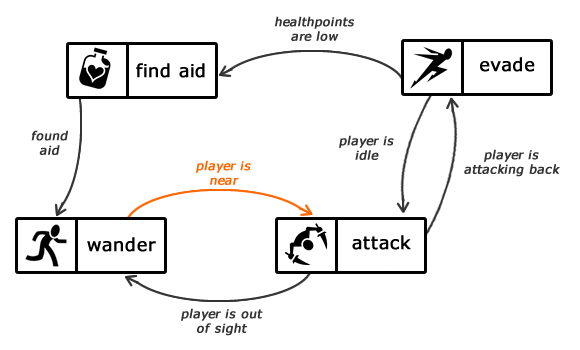
\includegraphics[width=\textwidth]{fsm_enemy_brain}
		% https://gamedevelopment.tutsplus.com/tutorials/finite-state-machines-theory-and-implementation--gamedev-11867
	\end{center}
\end{frame}

\begin{frame}{Behaviour trees}
	\begin{center}
		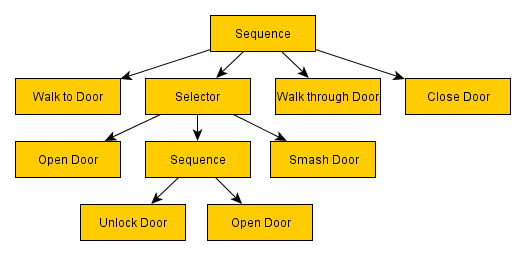
\includegraphics[width=\textwidth]{behaviour_tree}
		% https://www.gamasutra.com/blogs/ChrisSimpson/20140717/221339/Behavior_trees_for_AI_How_they_work.php
	\end{center}
\end{frame}

\begin{frame}{Game tree search}
	\begin{center}
		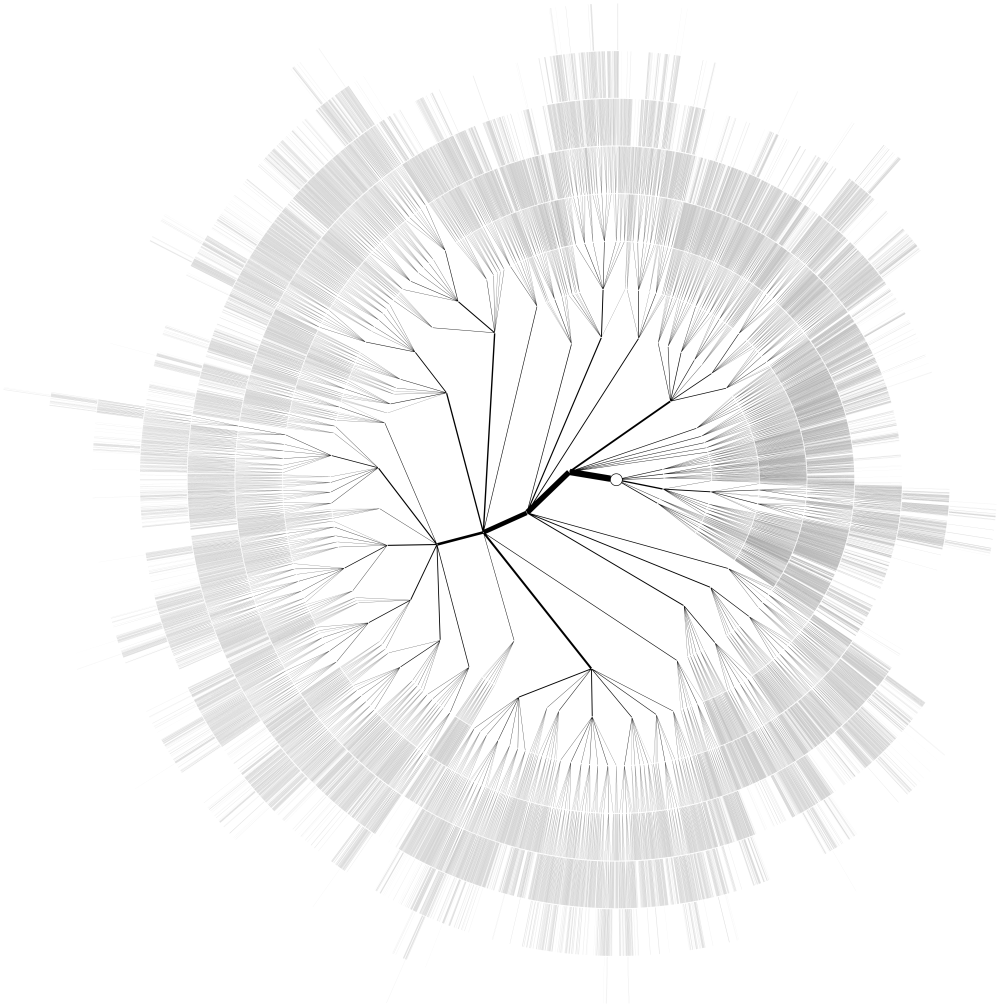
\includegraphics[height=0.7\textheight]{mcts}
	\end{center}
\end{frame}

\begin{frame}{Multi-agent approaches (e.g.\ flocking)}
	\begin{center}
		
\includegraphics[width=\textwidth]{flocking}
		% https://www.youtube.com/watch?v=5p6OAEVKw-0
	\end{center}
\end{frame}

\begin{frame}{Machine learning}
	\begin{center}
		\colorbox{white}{
			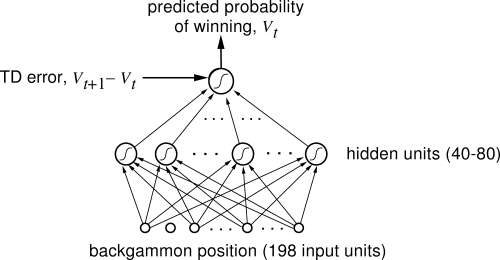
\includegraphics[width=0.7\textwidth]{tdgammon}
		}
		% https://users.auth.gr/kehagiat/Research/GameTheory/12CombBiblio/BackGammon.html
	\end{center}
\end{frame}

\begin{frame}{AI architectures}
	\begin{itemize}
		\pause\item Can roughly be divided into \textbf{hand-authored}...
			\begin{itemize}
				\pause\item Rule-based, FSM, behaviour trees
			\end{itemize}
		\pause\item ... and \textbf{computational intelligence}
			\begin{itemize}
				\pause\item Search, multi-agent, machine learning
			\end{itemize}
		\pause\item Do you want to \textbf{design} the AI behaviours yourself,
			or do you want them to \textbf{emerge} from the system?
		\pause\item Predictability and authorial control versus adaptability and novelty
		\pause\item Can also combine the two
			\begin{itemize}
				\pause\item E.g.\ use a rule-based system to constrain a CI system
				\pause\item E.g.\ flocking --- individual agents are usually rule-based, but overall flock dynamics
					are emergent
			\end{itemize}
	\end{itemize}
\end{frame}

\part{Finite state machines}
\frame{\partpage}

\begin{frame}{Finite state machines}
    \begin{itemize}
        \item A \textbf{finite state machine (FSM)} consists of: \pause
            \begin{itemize}
                \item A set of \textbf{states}; and \pause
                \item \textbf{Transitions} between states \pause
            \end{itemize}
        \item At any given time, the FSM is in a \textbf{single state} \pause
        \item \textbf{Inputs} or \textbf{events} can cause the FSM to transition to a different state
    \end{itemize}
\end{frame}

\begin{frame}{State transition diagrams}
    \begin{center}\scalebox{0.8}{
        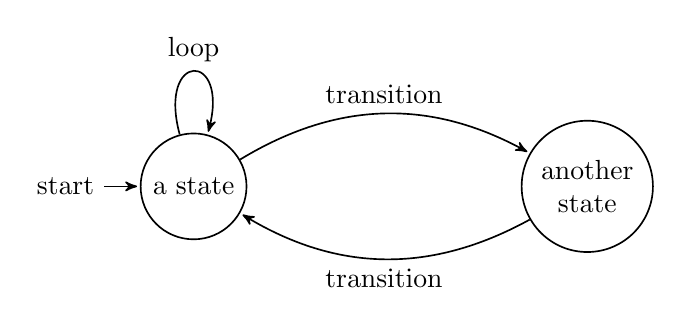
\begin{tikzpicture}[->,>=stealth',shorten >=1pt,auto,node distance=5cm,
                            semithick]
            \node[initial,state] (A) {a state};
            \node[state] (B) [right of=A, align=center] {another\\state};

            \path (A) edge [bend left] node [above] {transition} (B)
                  (B) edge [bend left] node [below] {transition} (A)
                  (A) edge [loop above] node {loop} (A);
        \end{tikzpicture}
    }\end{center}
    \begin{itemize}
        \item FSMs are often drawn as \textbf{state transition diagrams}
        \item Reminiscent of \textbf{flowcharts} and certain types of \textbf{UML diagram} \pause
    \end{itemize}
\end{frame}

\begin{frame}{FSMs for AI behaviour}
    The next slide shows a simple FSM for the following AI behaviour, for an enemy NPC in a shooter game: \pause
    \begin{itemize}
        \item By default, patrol (e.g.\ along a preset route) \pause
        \item If the player is spotted, attack them \pause
        \item If the player is no longer visible, resume patrolling \pause
        \item If you are low on health, run away and find a medikit. Then resume patrolling \pause
        \item If you are low on ammo, run away and find ammo. Then resume patrolling \pause
    \end{itemize}
\end{frame}

\begin{frame}
    \begin{center}\scalebox{0.8}{
        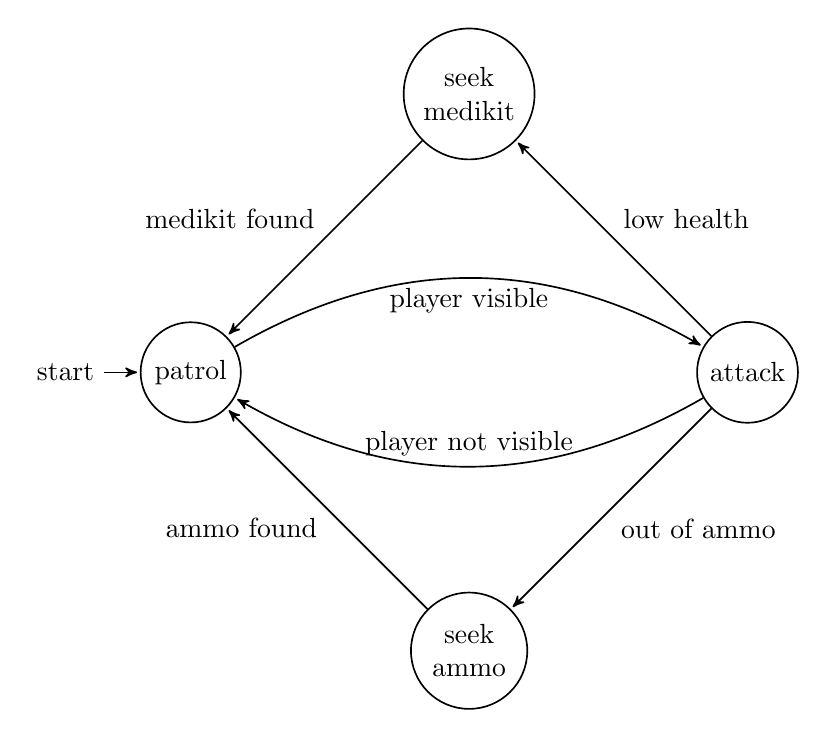
\begin{tikzpicture}[->,>=stealth',shorten >=1pt,auto,node distance=5cm,
                            semithick]
            \node[initial,state] (patrol) {patrol};
            \node[state] (health) [above right of=patrol, align=center] {seek\\medikit};
            \node[state] (ammo) [below right of=patrol, align=center] {seek\\ammo};
            \node[state] (attack) [above right of=ammo] {attack};

            \path (patrol) edge [bend left] node [below] {player visible} (attack)
                  (attack) edge [bend left] node [above] {player not visible} (patrol)
                  (attack) edge node [above right] {low health} (health)
                  (attack) edge node {out of ammo} (ammo)
                  (health) edge node [above left] {medikit found} (patrol)
                  (ammo) edge node {ammo found} (patrol);
        \end{tikzpicture}
    }\end{center}
\end{frame}

\begin{frame}{Other uses of FSMs}
    As well as AI behaviours, FSMs may also be used for: \pause
    \begin{itemize}
        \item Animation \pause
        \item UI menu systems \pause
        \item Dialogue trees \pause
        \item Token parsing \pause
        \item ...
    \end{itemize}
\end{frame}

\begin{frame}{Beyond FSMs}
    Some topics for you to research, for when plain old FSMs aren't enough... \pause
    \begin{itemize}
        \item Hierarchical FSMs
        \item Nested FSMs
        \item Stack-based FSMs
        \item Hierarchical task networks
        \item ...
    \end{itemize}
		Plus the topic we will be looking at today: \textbf{behaviour trees}
\end{frame}

\part{Behaviour Trees}
\frame{\partpage}

\begin{frame}{Behaviour trees (BTs)}
	\begin{itemize}
		\pause\item A \textbf{hierarchical} model of decision making
		\pause\item Allow \textbf{complex behaviours} to be built up from \textbf{simple components}
		\pause\item Allow for \textbf{more complex} behaviours than FSMs
		\pause\item First used in Halo 2 (2005), now used extensively
		\pause\item Also used in robotics and other non-game AI applications
	\end{itemize}
\end{frame}

\begin{frame}{Using BTs}
	\begin{itemize}
		\pause\item Fairly easy to implement; plenty of resources online
		\pause\item \textbf{Unreal}: an advanced BT system is built in
		\pause\item \textbf{Unity}: numerous free and paid options on the Asset Store
			e.g.\ Behavior Machine, Behavior Designer, Behave, RAIN
	\end{itemize}
\end{frame}

\begin{frame}{BT basics}
	\begin{itemize}
		\pause\item A BT is a \textbf{tree} of \textbf{nodes}
		\pause\item On each game update (i.e.\ each frame), the root node is \textbf{ticked}
			\begin{itemize}
				\pause\item When a node is ticked, it might cause some or all of its \textbf{children} to tick as well
				\pause\item So ticks propagate down the tree from the root
			\end{itemize}
		\pause\item A ticked node returns one of three \textbf{statuses}:
			\begin{itemize}
				\pause\item Success
				\pause\item Running
				\pause\item Failure
			\end{itemize}
		\pause\item ``Running'' status allows nodes to represent operations that \textbf{last multiple frames}
	\end{itemize}
\end{frame}

\begin{frame}{Node types}
	\begin{itemize}
		\pause\item There are \textbf{two main types} of BT node
		\pause\item \textbf{Leaf} nodes
			\begin{itemize}
				\pause\item No children
				\pause\item Represent \textbf{tasks} (i.e.\ the AI agent actually doing something)
			\end{itemize}
		\pause\item \textbf{Composite} nodes
			\begin{itemize}
				\pause\item One or more children
				\pause\item Control which of the children run on each tick
			\end{itemize}
	\end{itemize}
\end{frame}

\begin{frame}{Leaf nodes}
	\begin{itemize}
		\pause\item Represent \textbf{atomic actions}
			\begin{itemize}
				\pause\item I.e.\ actions which can't sensibly be broken down into smaller actions
			\end{itemize}
		\pause\item E.g.\ walk to, crouch, attack, open door
		\pause\item Status:
			\begin{itemize}
				\pause\item Success means ``the action is done''
				\pause\item Failure means ``the action cannot be done''
				\pause\item Running means ``the action is still in progress''
			\end{itemize}
		\pause\item Leaf nodes can also be used to represent \textbf{conditions}
			\begin{itemize}
				\pause\item E.g.\ ``is my health below 10\%?''
				\pause\item Returns success for true, failure for false
			\end{itemize}
		\pause\item ... although this is not recommended in Unreal ---
			conditionals should be implemented as \textbf{decorators} instead
	\end{itemize}
\end{frame}

\begin{frame}{Composite nodes: sequence}
	\begin{itemize}
		\pause\item Run each child, in order
		\pause\item If \textbf{any} child returns failure, stop and return failure
		\pause\item If \textbf{all} children return success, stop and return success
	\end{itemize}
	\pause
	{\footnotesize\Tree
		[.\fbox{Sequence}
			[.\fbox{Walk to chest} ]
			[.\fbox{Open chest} ]
			[.\fbox{Pick up loot} ]
			[.\fbox{Close chest} ]
		]
	}
\end{frame}

\begin{frame}{Sequence nodes and conditions}
	\begin{itemize}
		\pause\item A sequence node can be used like an \lstinline{if (cond1 && cond2)} statement
	\end{itemize}
	\pause
	{\footnotesize\Tree
		[.\fbox{Sequence}
			[.\fbox{Is health $< 10$?} ]
			[.\fbox{Am I near cover?} ]
			[.\fbox{Move to cover} ]
			[.\fbox{Use medkit} ]
		]
	}
\end{frame}

\begin{frame}{Composite nodes: selector}
	\begin{itemize}
		\pause\item Run each child, in order
		\pause\item If a child returns failure, move onto the next one
		\pause\item If \textbf{any} child returns success, stop and return success
	\end{itemize}
	\pause
	{\footnotesize\Tree
		[.\fbox{Selector}
			[.\fbox{Open chest} ]
			[.\fbox{Sequence}
				[.\fbox{Unlock chest} ]
				[.\fbox{Open chest} ]
			]
			[.\fbox{Smash chest} ]
		]
	}
\end{frame}

\begin{frame}{Selectors and priority}
	\begin{itemize}
		\pause\item Order of selector children represents the \textbf{priority} of different alternatives
	\end{itemize}
	\pause
	{\scriptsize\Tree
		[.\fbox{Selector}
			[.\fbox{Sequence}
				[.\fbox{Health $<$ 10?} ]
				[.\fbox{Run away} ]
			]
			[.\fbox{Sequence}
				[.\fbox{Player visible?} ]
				[.\fbox{Attack} ]
			]
			[.\fbox{Patrol} ]
		]
	}
\end{frame}

\begin{frame}{Sequence vs selector}
	\begin{itemize}
		\pause\item Sequence: perform a list of actions; if one of them fails then abandon the task
		\pause\item Selector: try a list of alternatives; stop once you find one that works
		\pause\item Sequence works like \lstinline{and}, selector works like \lstinline{or}
	\end{itemize}
\end{frame}

\begin{frame}{Other composite nodes}
	\begin{itemize}
		\pause\item Execute children in \textbf{random} order
		\pause\item Execute children in \textbf{parallel}
		\pause\item \textbf{Decorator} nodes
		\begin{itemize}
			\pause\item \textbf{Inverter}: if child returns success then return failure, and vice versa
			\pause\item \textbf{Repeater}: run the child a number of times, or forever
			\pause\item Most BT frameworks allow programmers to create custom decorator nodes
		\end{itemize}
		\pause\item Some BT frameworks allow programmers to create custom composite nodes
	\end{itemize}
\end{frame}

\begin{frame}{Blackboard}
	\begin{itemize}
		\pause\item It is often useful to \textbf{share} data between nodes
		\pause\item A \textbf{blackboard} (sometimes called a \textbf{data context}) allows this
		\pause\item Blackboard defines \textbf{variables}, which can be \textbf{read} and \textbf{written} by nodes
		\pause\item Some BT frameworks allow blackboards to be \textbf{local} to the AI agent, \textbf{shared} between several agents, or \textbf{global} to all agents
		\pause\item (Shared blackboards mean that your AI has ``telepathy'' --- this may or may not be desirable!)
	\end{itemize}
\end{frame}

\begin{frame}{BTs in The Division}
	\begin{center}
		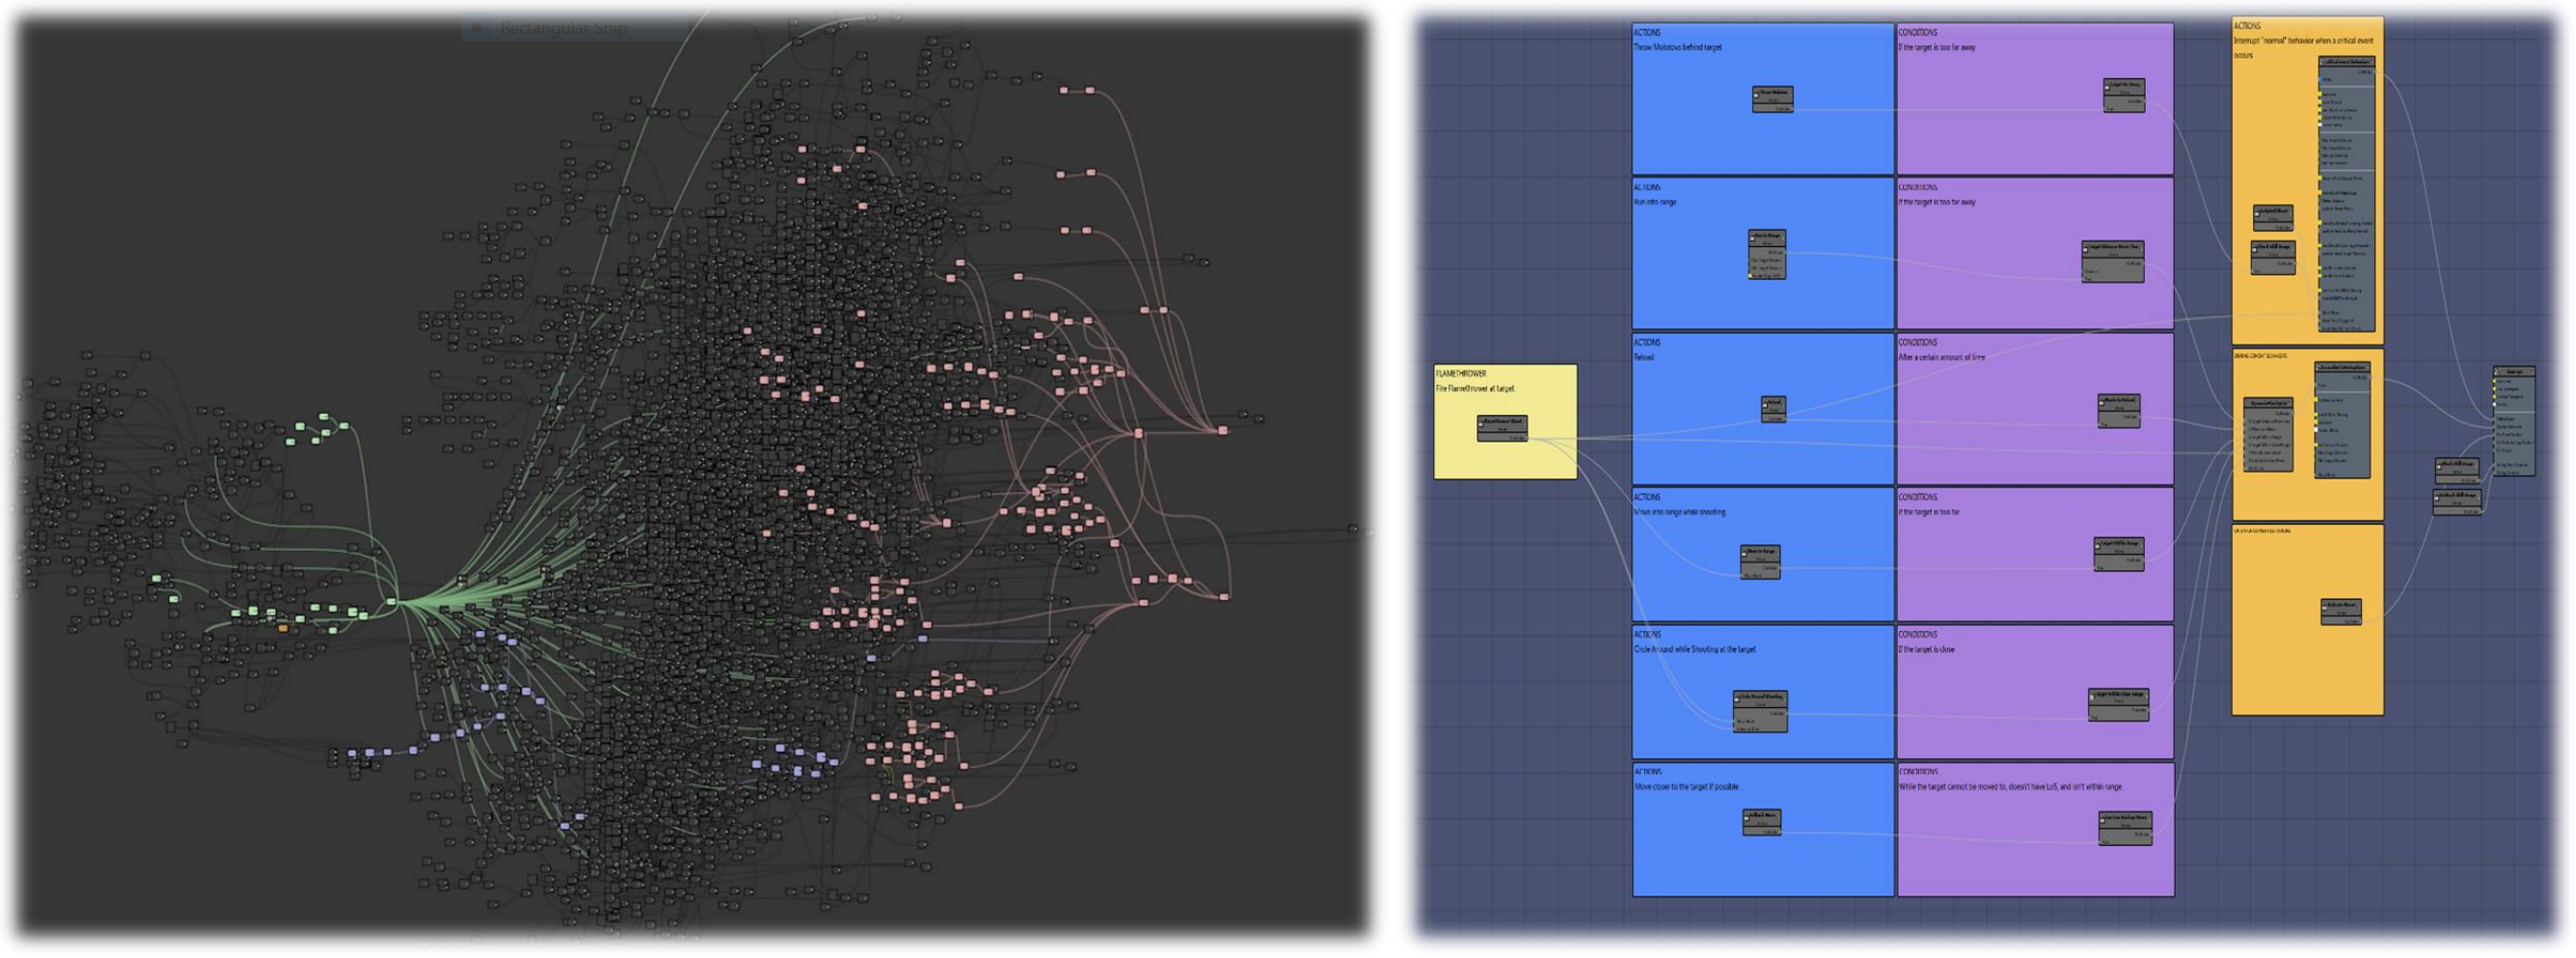
\includegraphics[width=\textwidth]{the_division}
		
		\url{http://www.gdcvault.com/play/1023382/AI-Behavior-Editing-and-Debugging}
	\end{center}
\end{frame}


\end{document}
